% ============================================================
% Tarea 01 — Reporte: Cursos de Cisco Packet Tracer
% (Introducción a Cisco Packet Tracer / Exploración de redes)
% Redes de Comunicaciones de Datos (6.º semestre)
% UAZ · Unidad Académica de Ingeniería Eléctrica
% ============================================================
\documentclass[11pt,a4paper]{article}

\usepackage[utf8]{inputenc}
\usepackage[T1]{fontenc}
\usepackage[spanish,mexico]{babel}
\usepackage{graphicx}
\usepackage[margin=2.5cm]{geometry}
\usepackage{setspace}
\usepackage{parskip}
\usepackage{fancyhdr}
\usepackage{pdfpages}
\usepackage[hidelinks]{hyperref}
\usepackage{xurl}

\onehalfspacing
\setlength{\parskip}{6pt}

\setlength{\headheight}{40pt}
\pagestyle{fancy}
\fancyhf{}
\fancyhead[L]{
\includegraphics[width=1cm]{../../../Assets/UIE.png}}
\fancyfoot[C]{\thepage}
\renewcommand{\headrulewidth}{0.4pt}

\begin{document}

% ---------------------------- PORTADA -----------------------
\begin{titlepage}
  \thispagestyle{empty}
  \begin{center}
    \vspace*{1cm}
    
\includegraphics[width=4.5cm]{../../../Assets/uaz.png}
    \vspace{0.8cm}

    {\large Universidad Autónoma de Zacatecas}\\[4pt]
    {\large Unidad Académica de Ingeniería Eléctrica}\\[4pt]
    {\normalsize Ingeniería Electrónica Industrial con especialidad en Telecomunicaciones}

    \vspace{1.8cm}
    {\LARGE\bfseries Tarea 01}\\[10pt]
    {\Large\bfseries Reporte de cursos de formación:\\[4pt] Introducción a Cisco Packet Tracer y\\ Exploración de redes con Cisco Packet Tracer}
  \end{center}

  \vspace{2.2cm}
  \begin{center}
    \begin{tabular}{rl}
      \textbf{Materia:} & Redes de Comunicaciones de Datos\\
      \textbf{Docente:} & José Ricardo Gómez Rodríguez\\
      \textbf{Alumno:}  & Arnold Yovick Ríos Zaldívar\\
      \textbf{Fecha:}   & Septiembre de 2026\\
    \end{tabular}
  \end{center}
  \vfill
\end{titlepage}

% ------------------------- INTRODUCCIÓN ---------------------
\section{Introducción}

Cisco Packet Tracer es el simulador de redes desarrollado por Cisco Networking
Academy que permite diseñar, configurar y diagnosticar topologías de red sin
contar con hardware físico. Su importancia en la formación en redes de datos
radica en que reproduce el comportamiento de dispositivos reales (routers,
switches, puntos de acceso, servidores y equipos finales) y hace visible lo que
en una red productiva permanece oculto: la encapsulación de los datos, el flujo
de paquetes y las respuestas de cada capa del modelo de referencia.

Como parte de la evaluación de la materia se completaron dos cursos oficiales
de Cisco Networking Academy, con una dedicación total estimada de cinco horas:

\begin{itemize}
  \item \textbf{Introducción a Cisco Packet Tracer}: familiarización con la
        interfaz, las herramientas y las funcionalidades básicas del software;
        creación de topologías simples, agregado de dispositivos, conexiones
        físicas y lógicas, y exploración de los espacios de trabajo lógico y
        físico.
  \item \textbf{Exploración de redes con Cisco Packet Tracer}: configuración
        básica de dispositivos de red, uso de la interfaz de línea de comandos
        (CLI), monitoreo de la red mediante el Controlador de Red y simulación
        del comportamiento de los paquetes conforme a los modelos OSI y TCP/IP.
\end{itemize}

El presente reporte documenta las actividades realizadas en ambos cursos, incluye
las capturas de pantalla que constituyen la evidencia del trabajo efectuado,
describe los comandos CLI empleados y explica el comportamiento de los paquetes
observado en el modo de simulación. Como constancia de la finalización de ambos
cursos, se anexan los certificados oficiales emitidos por Cisco Networking
Academy (Anexo~A).

% -------------------------- OBJETIVOS -----------------------
\section{Objetivos}

\subsection{Objetivo general}

Completar los cursos \textit{Introducción a Cisco Packet Tracer} y
\textit{Exploración de redes con Cisco Packet Tracer} de Cisco Networking
Academy, adquiriendo las competencias básicas para simular, configurar y
diagnosticar redes de datos.

\subsection{Objetivos específicos}

\begin{itemize}
  \item Familiarizarse con la interfaz, las herramientas y los espacios de
        trabajo (lógico y físico) de Cisco Packet Tracer.
  \item Crear topologías simples agregando dispositivos finales, switches,
        routers y enlaces de distintos tipos.
  \item Emplear el espacio de trabajo físico para modelar cableado
        estructurado, racks y conectividad inalámbrica y celular.
  \item Ejecutar comandos de la CLI para configurar y verificar dispositivos
        de red.
  \item Analizar, mediante el modo de simulación, el flujo de paquetes y su
        relación con los modelos OSI y TCP/IP.
\end{itemize}

% -------------------------- DESARROLLO ----------------------
\section{Desarrollo}

\subsection{Curso 1: Introducción a Cisco Packet Tracer}

El primer curso se centró en el manejo del entorno de trabajo. Se exploraron
los elementos principales de la interfaz: la barra de menús, la paleta de
tipos de dispositivos (equipos finales, switches, routers, puntos de acceso y
dispositivos de cableado), la paleta de conexiones (cables directos, cruzados,
de fibra, seriales y de consola), y los dos espacios de trabajo que ofrece la
herramienta. En el \textbf{espacio lógico} se construyen las topologías y se
configuran los dispositivos; en el \textbf{espacio físico} se modela el
entorno real de instalación: ciudades, edificios, oficinas, racks y armarios
de cableado.

Como práctica inicial se construyó una topología básica en el espacio lógico,
integrando un router inalámbrico, la nube de Internet y un servidor
(\texttt{cisco.srv}), unidos mediante enlaces cobre; durante la actividad se
verificó que los indicadores de enlace en verde señalizan conexiones
operativas en ambos extremos (Figura~\ref{fig:redsimple}).

\begin{figure}[htbp]
  \centering
  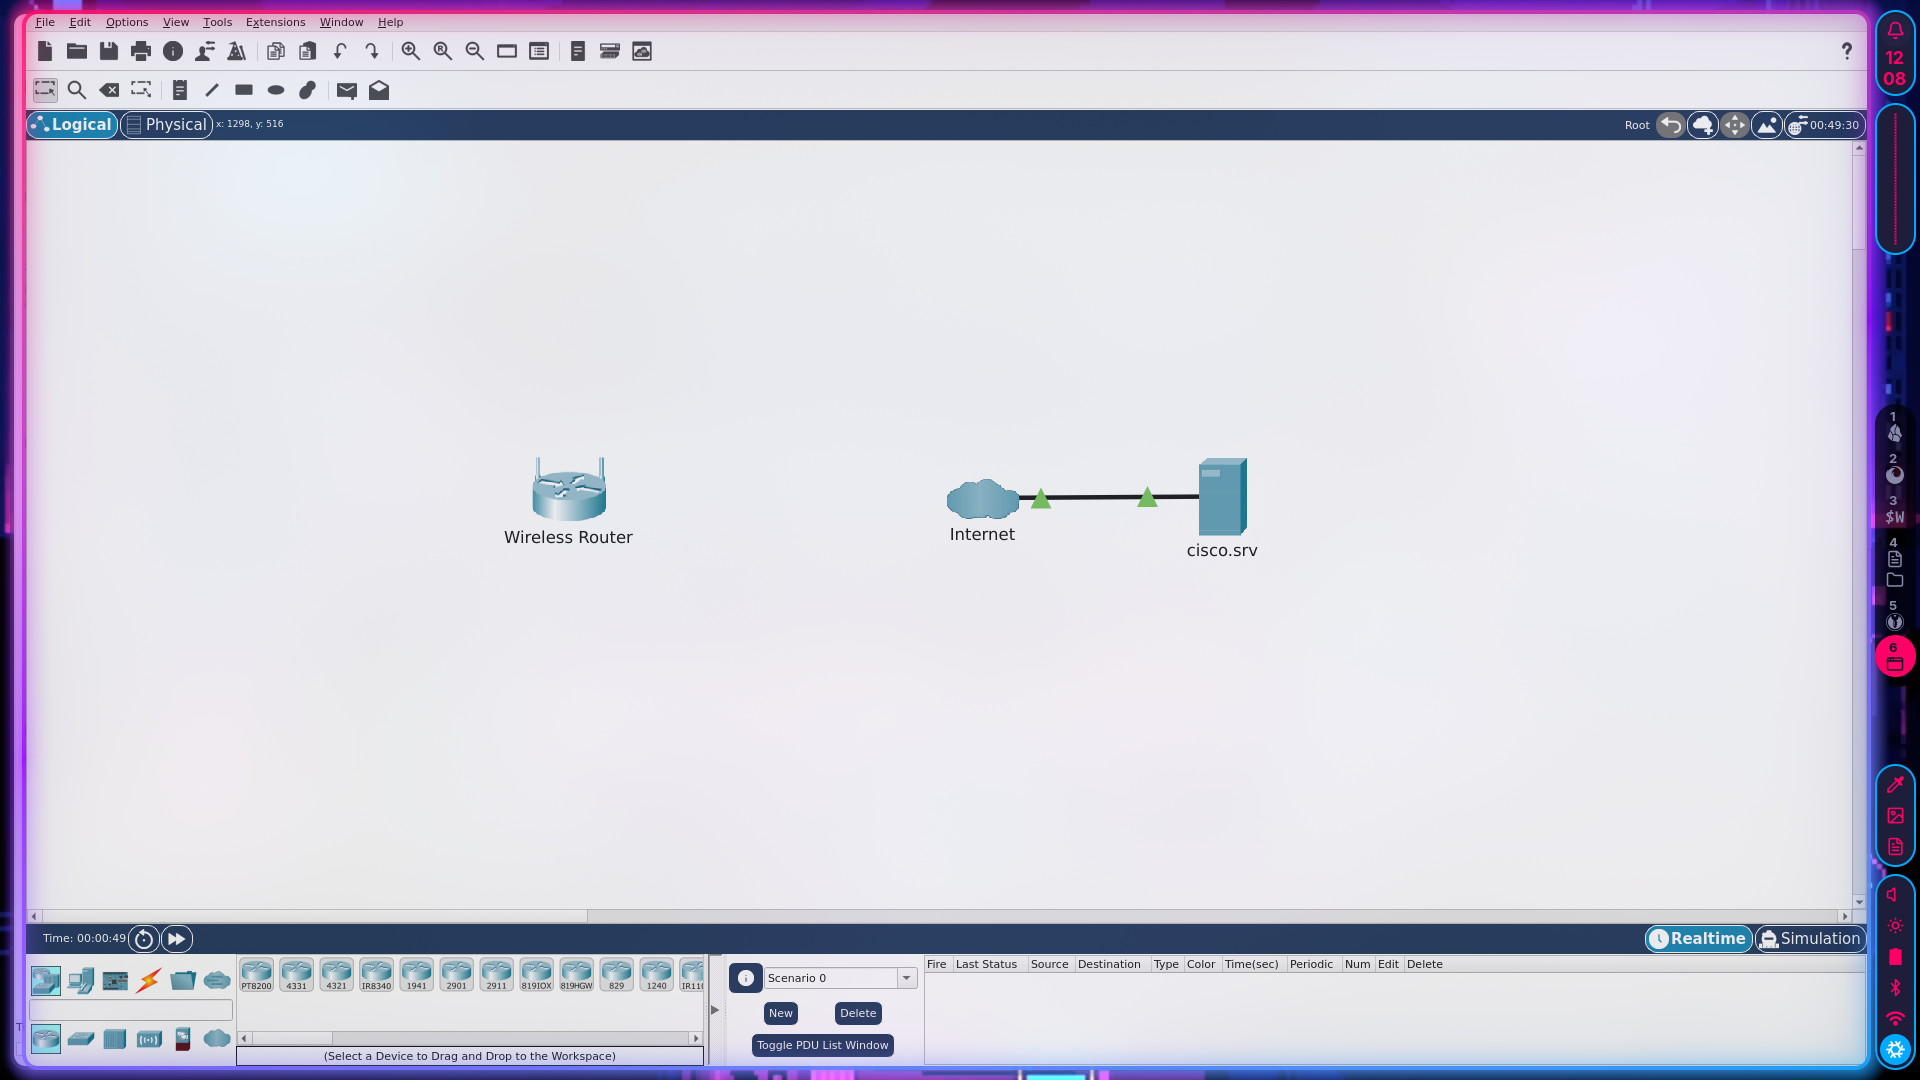
\includegraphics[width=0.85\textwidth]{../img/redSimple.png}
  \caption{Topología básica en el espacio lógico: router inalámbrico, nube de
  Internet y servidor \texttt{cisco.srv} conectados mediante enlaces cobre
  operativos.}
  \label{fig:redsimple}
\end{figure}

Posteriormente se trabajó en el espacio de trabajo físico, explorando la vista
de una oficina con equipos finales (laptop, smartphone, tableta e impresora).
En la actividad correspondiente se ancló una computadora portátil a una red
celular a través de un teléfono inteligente: se habilitó Bluetooth en la
laptop, se activó el anclaje celular (\textit{cellular tethering}) en el
smartphone y se verificó que este obtuviera dirección IP de la red celular
3G/4G, para finalmente emparejar ambos dispositivos por Bluetooth y dar acceso
web a la laptop mediante la conexión compartida (Figura~\ref{fig:conectar}).

\begin{figure}[htbp]
  \centering
  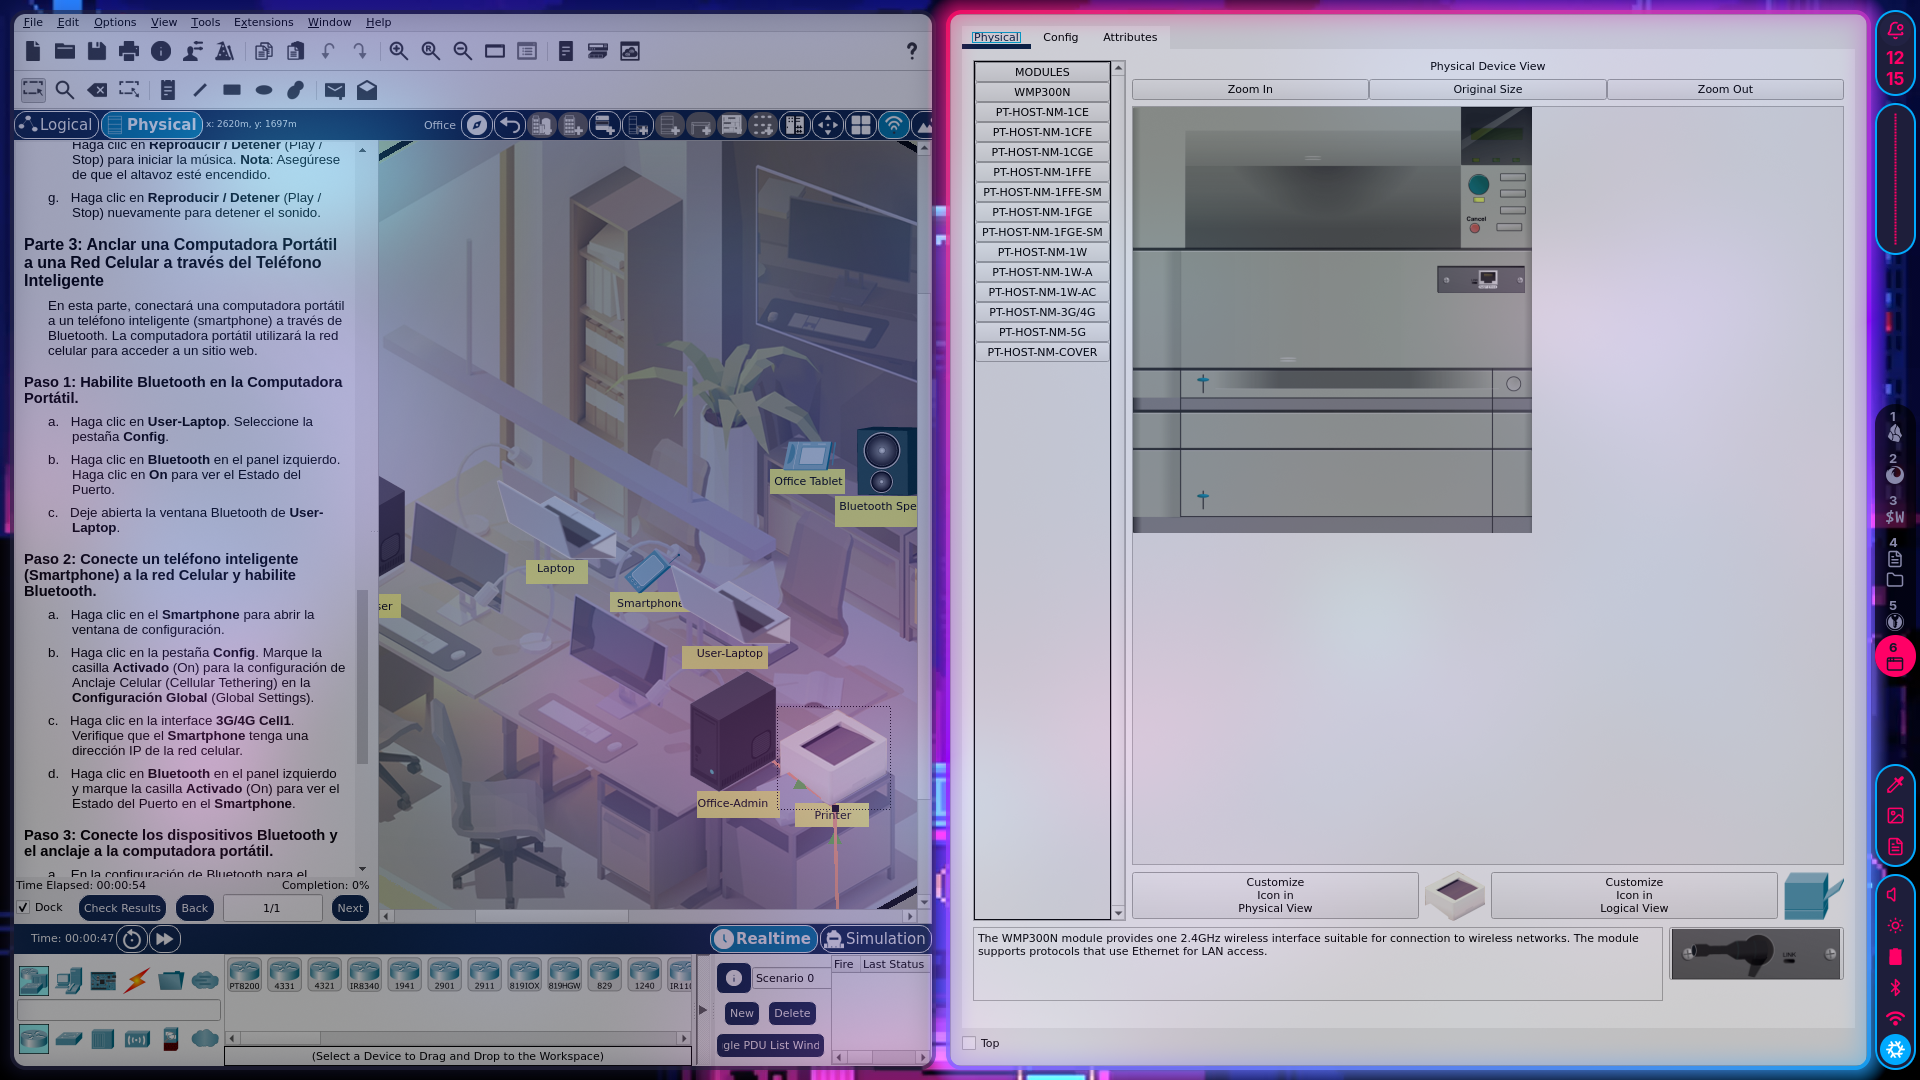
\includegraphics[width=0.85\textwidth]{../img/conectarDisp.png}
  \caption{Espacio de trabajo físico: oficina con laptop, smartphone, tableta
  e impresora durante la actividad de anclaje de la portátil a la red celular
  vía Bluetooth.}
  \label{fig:conectar}
\end{figure}

La tercera práctica abordó el cableado estructurado en el espacio físico. Se
instaló un panel de conexiones (\textit{patch panel}) en el armario de
cableado, se colocó un soporte de pared en la oficina y se tendieron los
cables que conectan los dispositivos de red de la oficina con el rack,
siguiendo las partes definidas en la actividad (Figura~\ref{fig:cableado}).
Esta práctica permitió comprender la correspondencia entre la topología
lógica de una red y su infraestructura física: paneles, soportes, canaletas y
racks. Adicionalmente se exploró la vista física de los dispositivos, donde es
posible inspeccionar y agregar módulos de hardware (por ejemplo, el módulo
inalámbrico WMP300N) con el equipo apagado, tal como se haría con una tarjeta
real.

\begin{figure}[htbp]
  \centering
  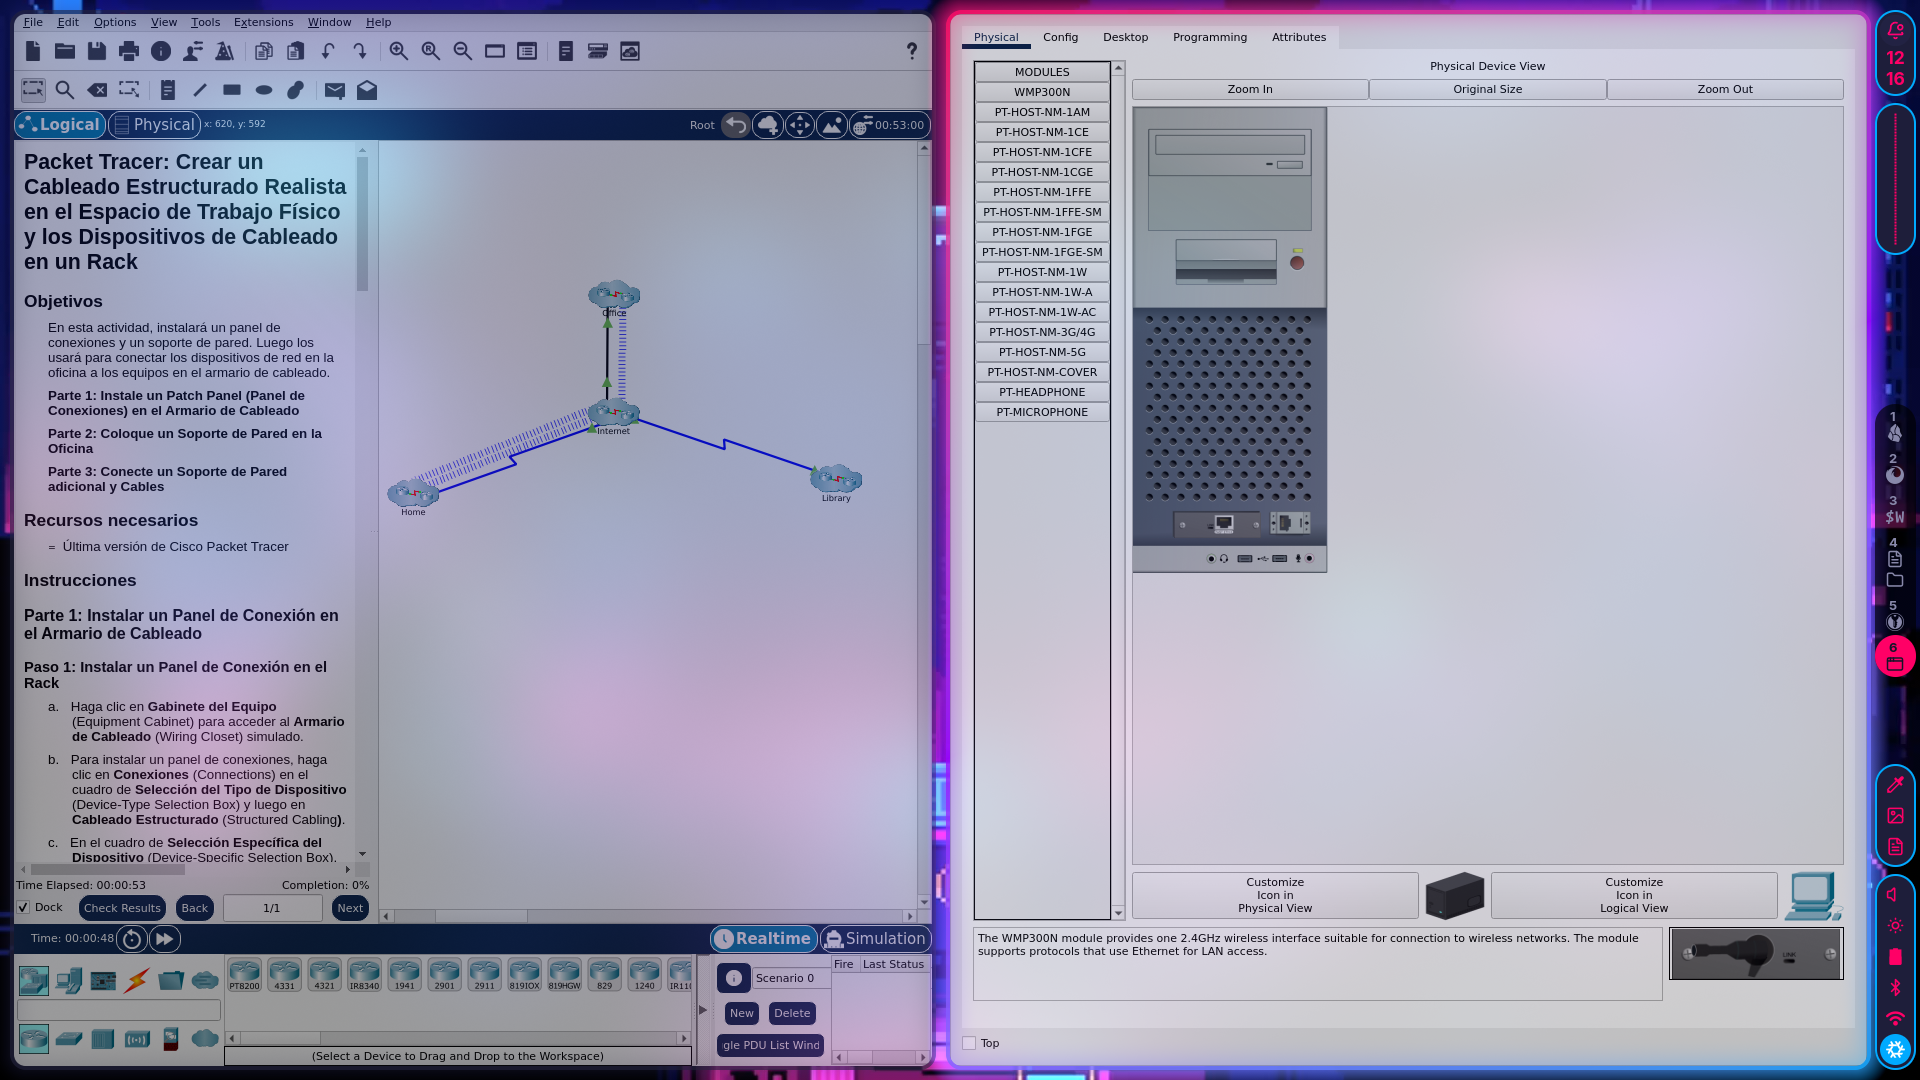
\includegraphics[width=0.85\textwidth]{../img/crearCableado.png}
  \caption{Actividad de cableado estructurado: topología entre Office,
  Library y Home (izquierda) y vista física del dispositivo con la bandeja de
  módulos de hardware disponible (derecha).}
  \label{fig:cableado}
\end{figure}

\subsection{Curso 2: Exploración de redes con Cisco Packet Tracer}

El segundo curso profundizó en la operación de la red ya construida: la
configuración de dispositivos, la verificación de conectividad y el análisis
del tráfico. La práctica central consistió en supervisar la red de una oficina
administrada por un \textbf{Controlador de Red} (\textit{Network
Controller}), elemento centralizado desde el cual se aprovisionan y monitorean
los equipos.

La topología de la práctica (Figura~\ref{fig:supervise}) integra un switch
principal (Office-SW1) con dos switches de acceso (Office-SW2, Office-SW3), un
router (Office-RT), un controlador inalámbrico (WLC) con su punto de acceso
ligero (LAP), un servidor, una impresora y equipos finales cableados e
inalámbricos (Office-Admin, Office-User, Office-Tablet y Smartphone), además
del propio Network Controller. Sobre esta red se realizaron tres actividades:

\begin{itemize}
  \item \textbf{Exploración del tablero (Dashboard)} del Controlador de Red,
        identificando los menús de aprovisionamiento (\textit{Provisioning}),
        aseguramiento (\textit{Assurance}) y los dispositivos visibles.
  \item \textbf{Documentación de la red}: mediante la función de notas se
        rotularon los dispositivos de red con su dirección IP de gestión, por
        ejemplo \texttt{Office-SW1: 192.168.20.4}, práctica esencial para el
        mantenimiento de una red.
  \item \textbf{Descubrimiento de hosts}: se conectaron la tableta y el
        smartphone a la red inalámbrica, verificando que ambos obtuvieran por
        DHCP una dirección del rango \texttt{192.168.2.x/24}; después, desde
        el Controlador de Red, se ejecutó el proceso de detección
        (\textit{Discovery}), observando cómo los hosts recién conectados
        aparecen en las pantallas HOSTS y DISCOVERY.
\end{itemize}

\begin{figure}[htbp]
  \centering
  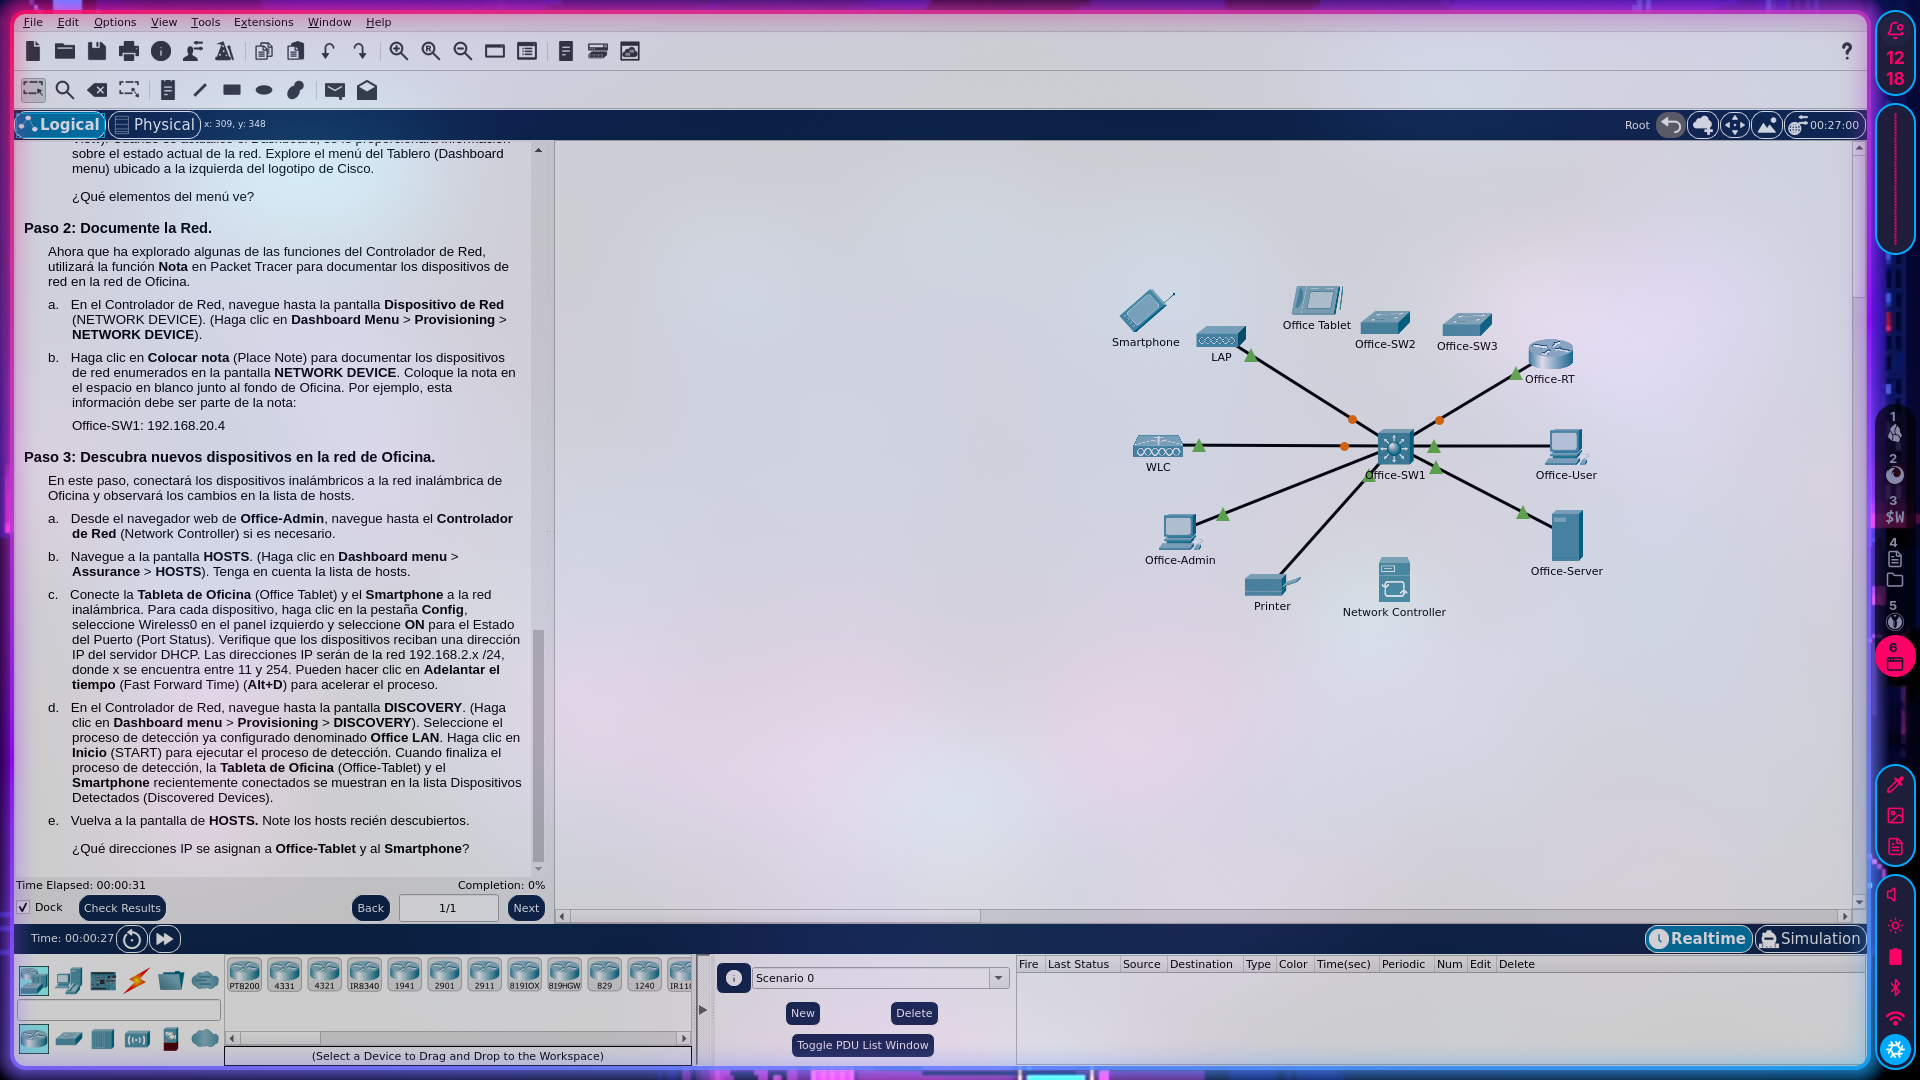
\includegraphics[width=0.95\textwidth]{../img/superviseRed.png}
  \caption{Red de oficina supervisada por el Controlador de Red: switches de
  acceso y distribución, router, WLC, punto de acceso ligero, Network
  Controller y hosts cableados e inalámbricos con direccionamiento DHCP.}
  \label{fig:supervise}
\end{figure}

\subsection{Configuración y verificación mediante la CLI}

A lo largo del segundo curso se utilizó la interfaz de línea de comandos tanto
en la pestaña \textit{Desktop} de los equipos finales como en la pestaña CLI
de los dispositivos de red. Los comandos empleados, con su propósito, se
resumen en la Tabla~\ref{tab:cli}.

\begin{table}[htbp]
  \centering
  \begin{tabular}{p{5.2cm}p{9.2cm}}
    \hline
    \textbf{Comando} & \textbf{Propósito} \\ \hline
    \texttt{ipconfig} / \texttt{ipconfig /all} & Verificar la configuración IP del host (dirección, máscara, gateway y servidores DHCP/DNS). \\
    \texttt{ping <destino>} & Probar la conectividad de capa 3 con un equipo remoto y medir el tiempo de ida y vuelta. \\
    \texttt{tracert <destino>} & Conocer la ruta (saltos) que siguen los paquetes hasta el destino. \\
    \texttt{nslookup} & Resolver nombres de dominio hacia direcciones IP consultando al servidor DNS. \\
    \texttt{enable} & Entrar al modo EXEC privilegiado del dispositivo Cisco. \\
    \texttt{configure terminal} & Entrar al modo de configuración global. \\
    \texttt{hostname <nombre>} & Asignar un nombre identificativo al dispositivo. \\
    \texttt{show ip interface brief} & Resumen del estado de las interfaces (IP asignada y estado up/down). \\
    \texttt{show running-config} & Mostrar la configuración activa del equipo. \\
    \texttt{copy running-config startup-config} & Guardar la configuración activa en la memoria de arranque. \\ \hline
  \end{tabular}
  \caption{Comandos CLI utilizados durante el curso para configurar y
  verificar los dispositivos de la red simulada.}
  \label{tab:cli}
\end{table}

El uso de estos comandos permite diagnosticar de manera sistemática: primero
se valida la configuración local del host (\texttt{ipconfig}), después la
conectividad hacia el gateway y equipos remotos (\texttt{ping}), y en caso de
falla se localiza el punto problemático inspeccionando la ruta
(\texttt{tracert}) o el estado de las interfaces del dispositivo
(\texttt{show ip interface brief}).

\subsection{Comportamiento de los paquetes y modelos OSI y TCP/IP}

Una de las aportaciones más valiosas del curso fue el uso del \textbf{modo de
simulación}, en el cual Packet Tracer muestra cada paquete como una
sobre (\textit{PDU}, Unidad de Datos de Protocolo) que viaja entre dispositivos
y permite inspeccionar, capa por capa, su contenido. Durante una petición web
sencilla (navegador de un PC hacia un servidor HTTP) se observó el proceso
completo de encapsulación descrito por el modelo:

\begin{enumerate}
  \item \textbf{Aplicación (capas 5--7)}: el navegador genera la petición HTTP
        hacia el servidor; antes de poder enviarla, se resuelve el nombre del
        servidor mediante DNS y, si no se conoce la MAC del siguiente salto,
        se emite una solicitud ARP.
  \item \textbf{Transporte (capa 4)}: la petición se segmenta y se agregan los
        puertos de origen y destino (TCP 80 para HTTP, UDP 53 para DNS),
        estableciendo la sesión confiable correspondiente.
  \item \textbf{Red (capa 3)}: a cada segmento se le adjunta la cabecera IP
        con las direcciones lógicas de origen y destino; la PDU resultante es
        un paquete.
  \item \textbf{Enlace (capa 2)}: el paquete se encapsula en una trama con las
        direcciones MAC de origen y del siguiente salto, que cambian en cada
        router intermedio aunque las direcciones IP permanezcan constantes.
  \item \textbf{Física (capa 1)}: la trama se convierte en bits y se
        transmite por el medio (cobre o radiofrecuencia en los enlaces
        inalámbricos).
\end{enumerate}

En el equipo destino el proceso se invierte (desencapsulación) y la petición
asciende hasta la aplicación, que responde con el flujo de regreso. La
visualización capa por capa evidenció la correspondencia entre ambos modelos:
mientras TCP/IP es el conjunto de protocolos realmente implementado en la
red, el modelo OSI sirve como referencia para localizar en qué capa ocurre una
falla (por ejemplo, un enlace mal conectado es un problema de capa 1, una MAC
incorrecta de capa 2, y una dirección IP errónea de capa 3), lo que convierte
el diagnóstico en un procedimiento ordenado.

% --------------------- SÍNTESIS REFLEXIVA -------------------
\section{Síntesis reflexiva de competencias adquiridas}

La suma de cinco horas de formación, distribuidas en ambos cursos, produjo un
aprendizaje que va más allá del manejo de una herramienta concreta.

En el plano instrumental, se dominó el flujo de trabajo completo de Packet
Tracer: seleccionar dispositivos, conectarlos con el medio adecuado (aprendiendo
a distinguir cables directos de cruzados, y cuándo usar cada uno), configurar
direcciones IP desde pestañas gráficas o desde la CLI, y verificar el
resultado con utilerías estándar. La práctica de cableado estructurado dejó
una lección que suele pasarse por alto: toda red lógica descansa sobre una
infraestructura física que debe planificarse (racks, paneles, soportes y
etiquetado), y las herramientas de simulación actuales permiten modelarla con
realismo.

En el plano conceptual, el modo de simulación transformó la forma de entender
el tráfico de red: observar la trama ARP precediendo al primer paquete HTTP, o
las direcciones MAC cambiando de salto en salto mientras las IP se mantienen,
convierte abstracciones de aula en evidencia visual. Comprender la
encapsulación por capas no es un ejercicio teórico: es la base del
diagnóstico, pues indica dónde buscar cuando algo falla.

Finalmente, en el plano metodológico, se adquirió disciplina de documentación
y verificación: rotular dispositivos, registrar sus direcciones de gestión y
confirmar cada paso con comandos de verificación antes de continuar. Estas
competencias son directamente transferibles al trabajo con equipos reales y
constituyen la base para las prácticas posteriores de la materia, que abordarán
el enrutamiento, la conmutación y el diseño de infraestructuras de mayor
complejidad.

% -------------------------- CONCLUSIÓN ----------------------
\section{Conclusión}

Se completaron satisfactoriamente los cursos \textit{Introducción a Cisco
Packet Tracer} y \textit{Exploración de redes con Cisco Packet Tracer} de
Cisco Networking Academy, con una dedicación aproximada de cinco horas y la
emisión de los certificados de finalización correspondientes (fechados el 22
y 23 de agosto de 2026, incluidos en el Anexo~A).

La formación cumplió cada uno de los objetivos planteados: se dominó la
interfaz y los espacios de trabajo lógico y físico; se construyeron topologías
con dispositivos finales, routers y switches; se modeló cableado estructurado
con racks y paneles; se configuró y verificó una red de oficina administrada
por un Controlador de Red empleando comandos CLI; y se analizó el flujo de
paquetes en el modo de simulación, comprendiendo la encapsulación y el papel
de cada capa de los modelos OSI y TCP/IP. Con estos cursos queda establecida
la base práctica necesaria para las prácticas de diseño e implementación de
infraestructuras de red más avanzadas de la materia.

% --------------------------- ANEXO --------------------------
\appendix
\section{Anexo A: Certificados de finalización}

Se incluyen a continuación los certificados oficiales emitidos por Cisco
Networking Academy, como evidencia de la finalización de ambos cursos:

\begin{itemize}
  \item \textit{Introducción a Cisco Packet Tracer} --- finalizado el 22 de
        agosto de 2026 (Cert ID: \url{7721d84e-9de7-49cb-a27e-7f96e36d4603}).
  \item \textit{Exploración de redes con Cisco Packet Tracer} --- finalizado
        el 23 de agosto de 2026
        (Cert ID: \url{1b5cf991-6ef2-4826-bbad-a374a0fbf755}).
\end{itemize}

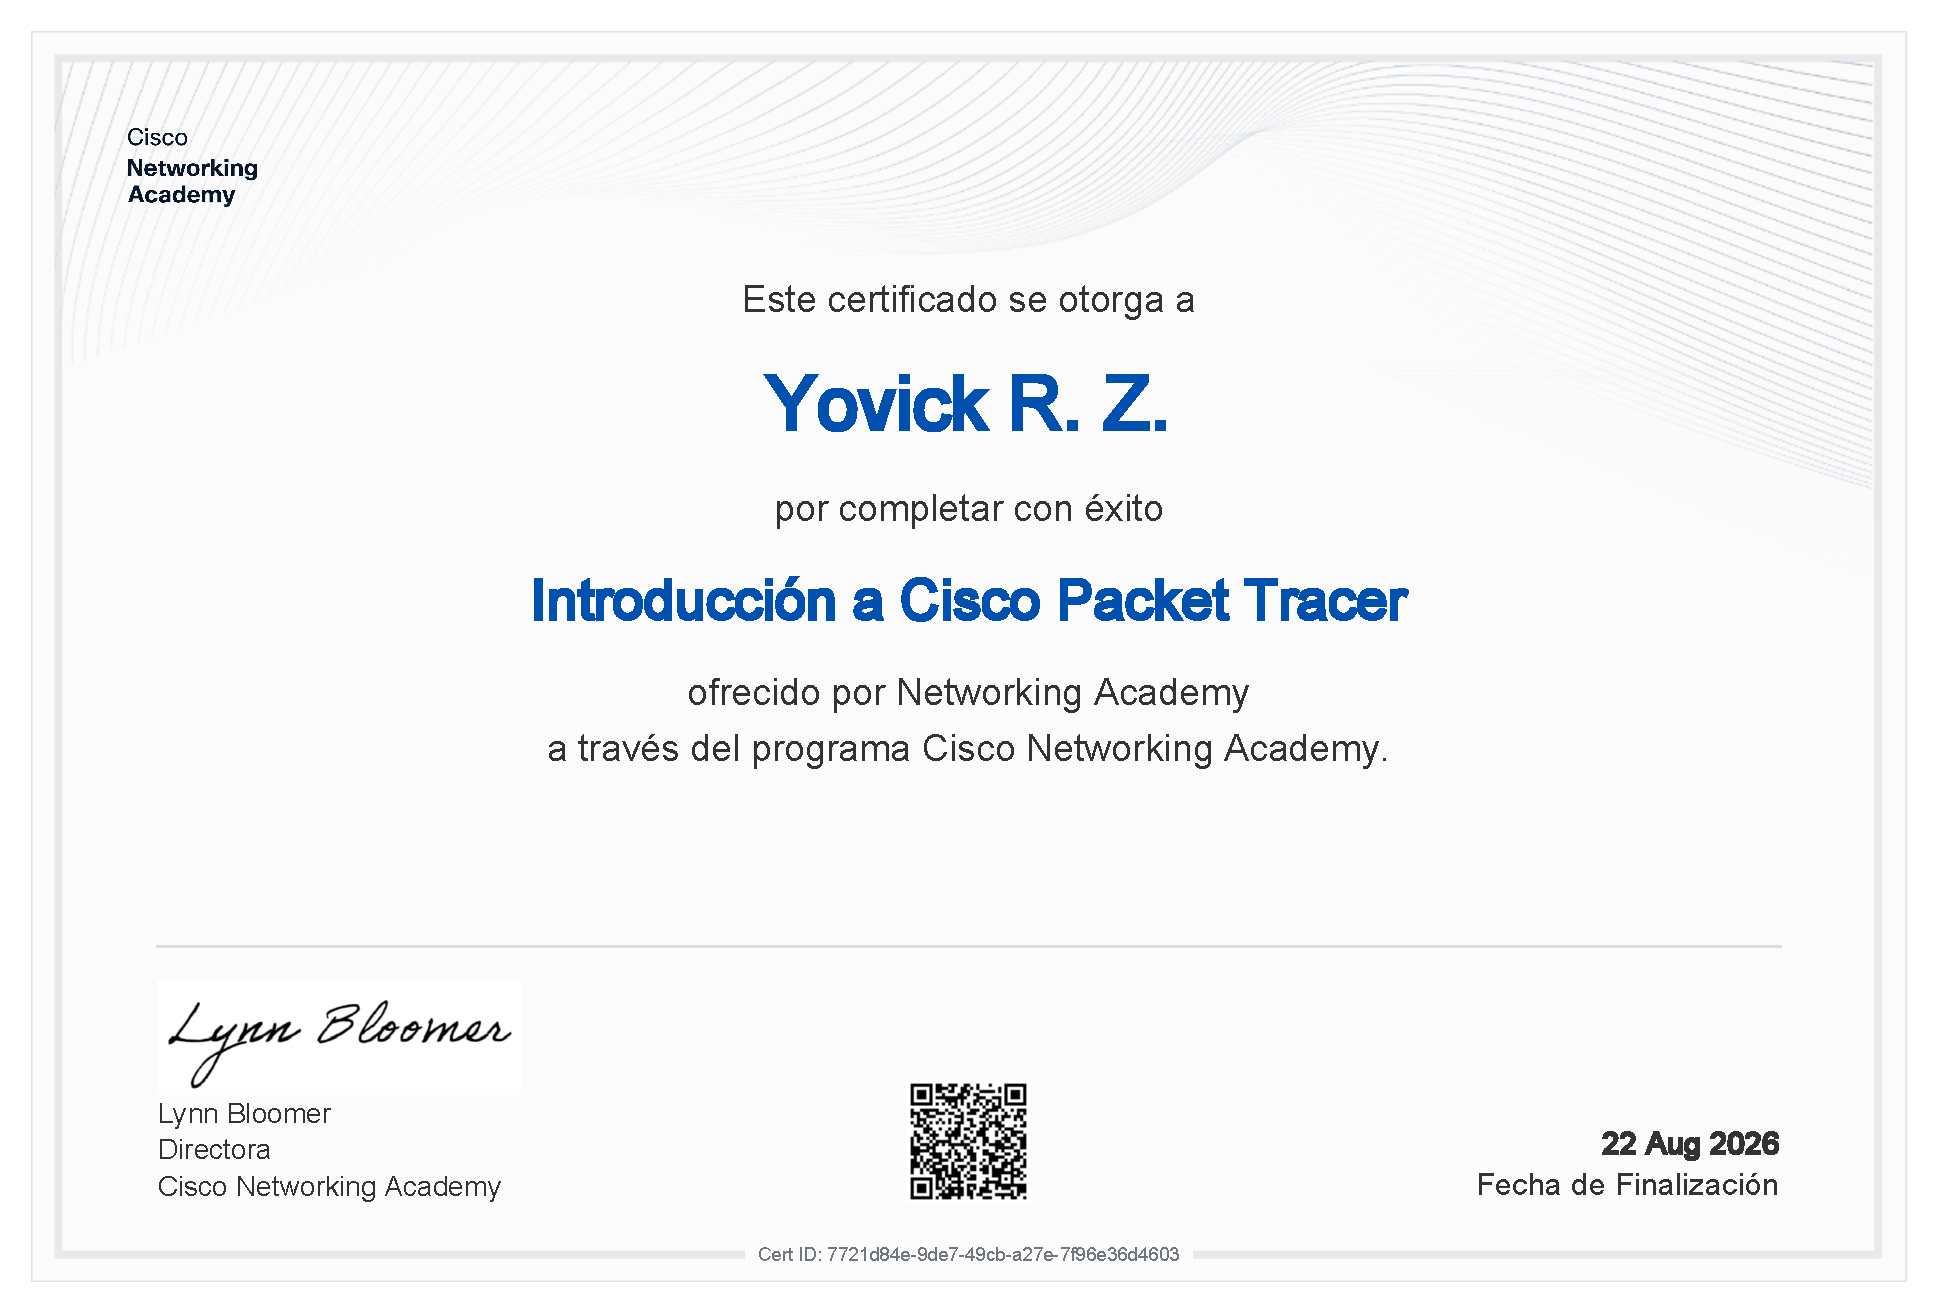
\includepdf[pages=-,pagecommand={\thispagestyle{fancy}}]{IntroductionCiscoPacketTracer.pdf}
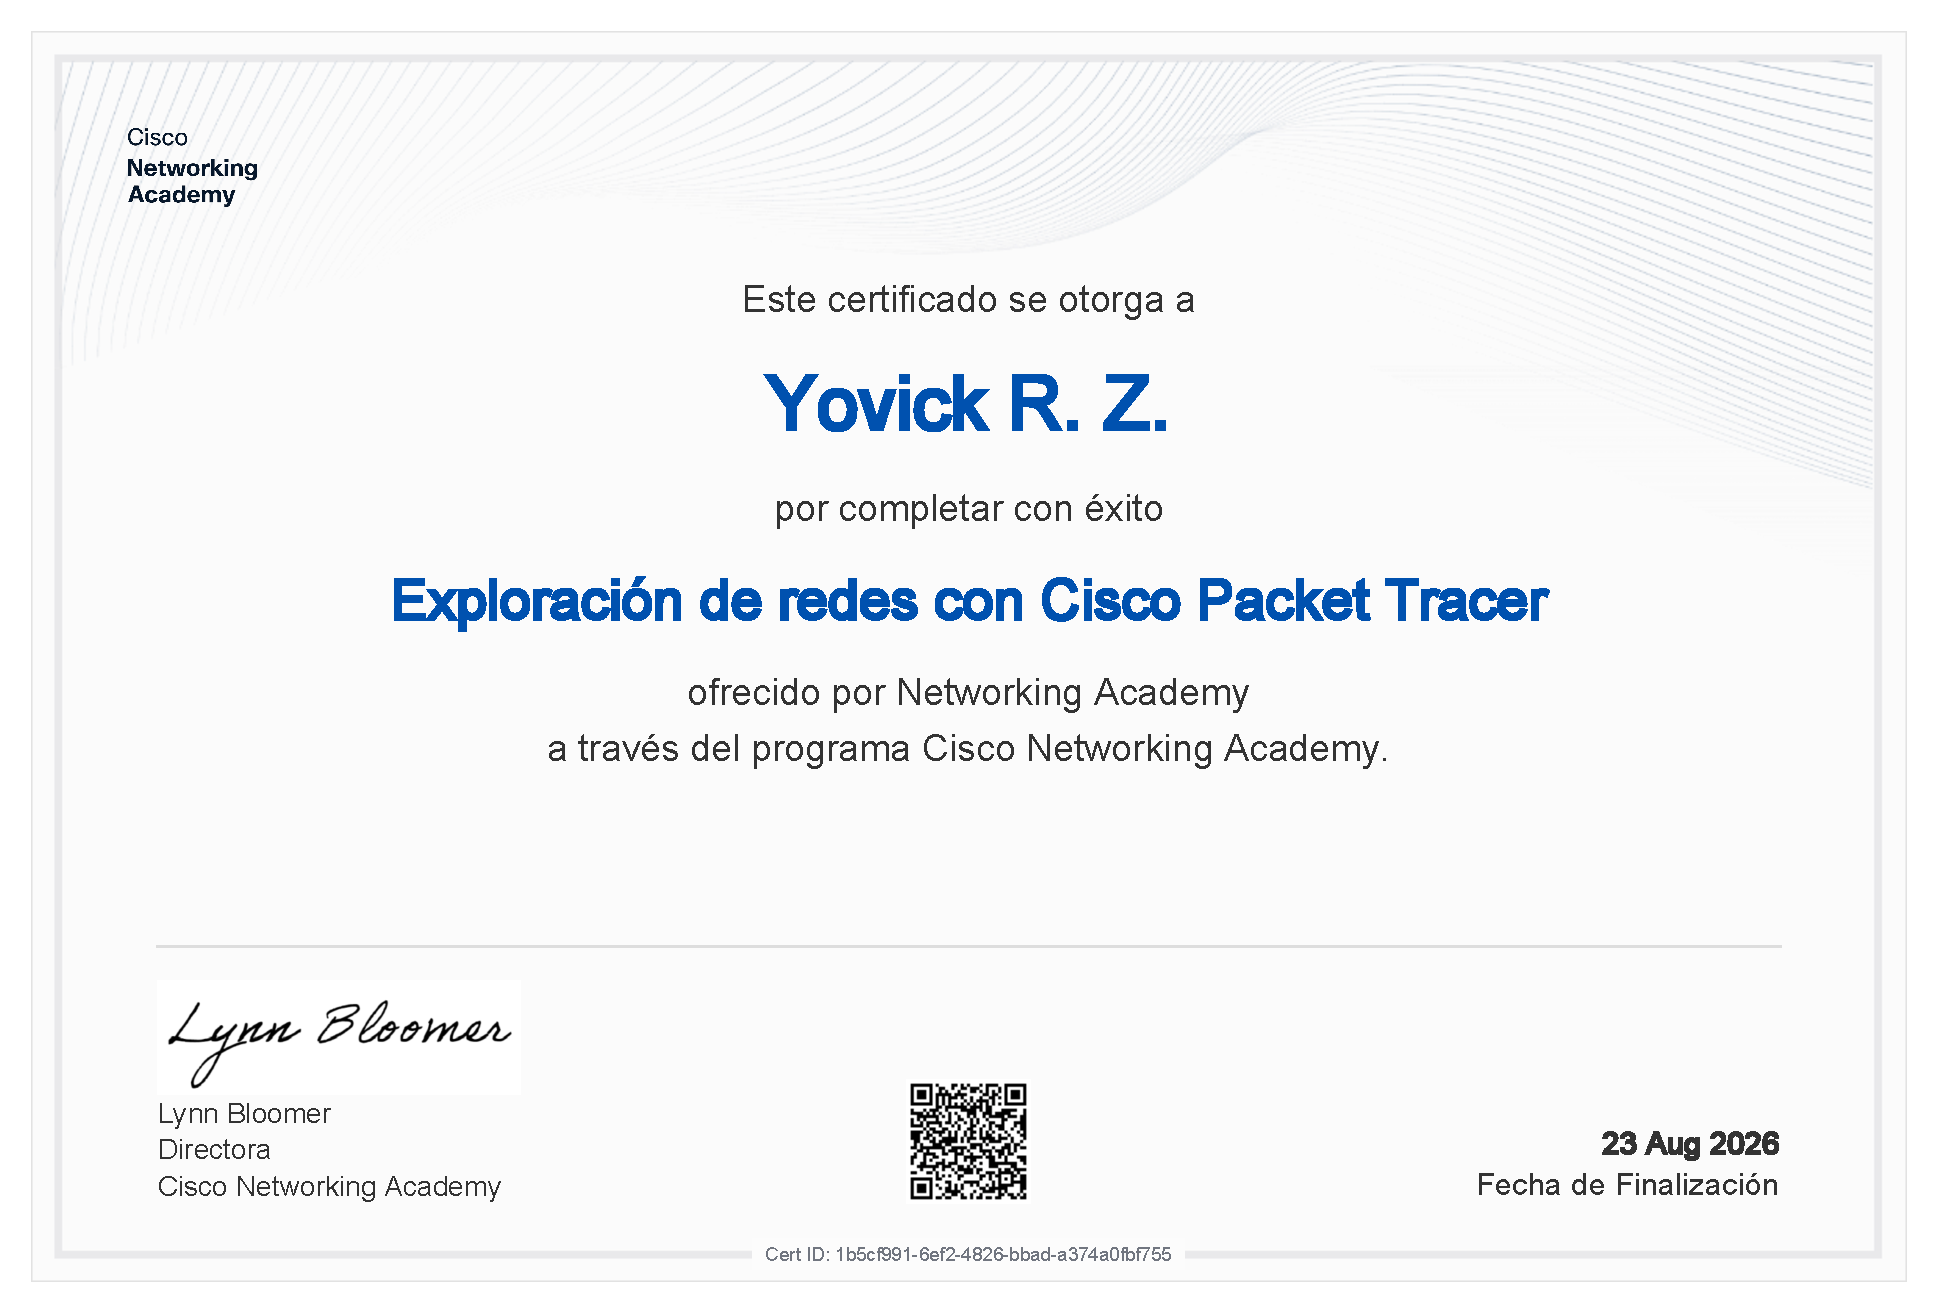
\includepdf[pages=-,pagecommand={\thispagestyle{fancy}}]{Exploring_Networking_with_Cisco_Packet_Tracer.pdf}

\end{document}
